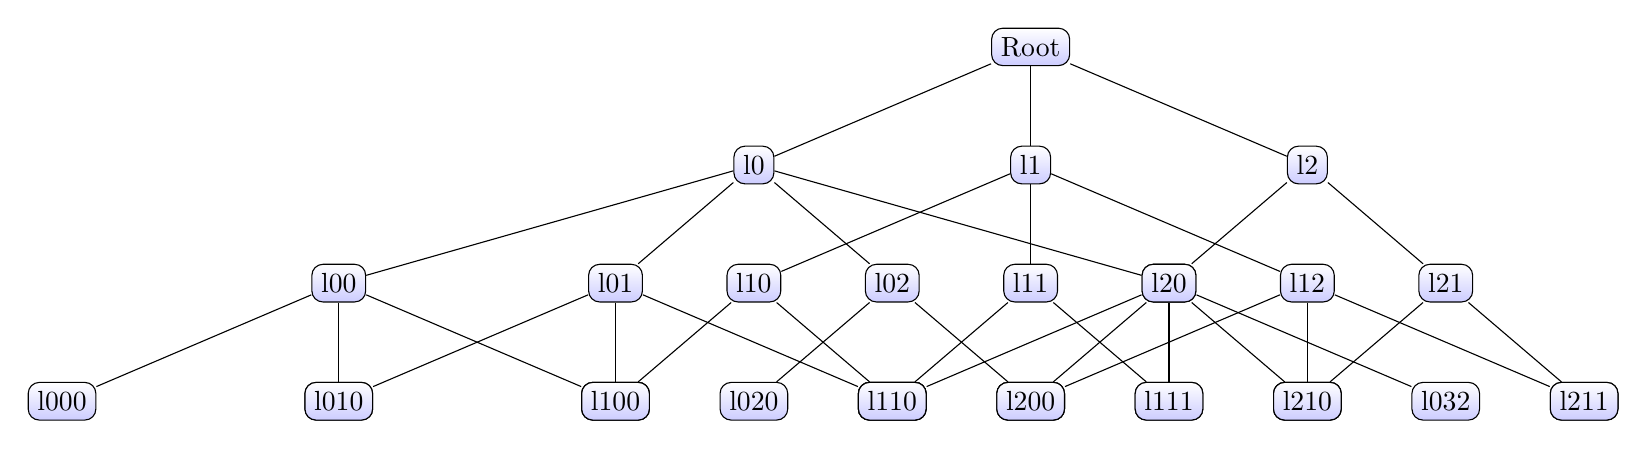
\begin{tikzpicture}[sibling distance=10em, every node/.style = {shape=rectangle, rounded corners, draw, align=center,top color=white, bottom color=blue!20}]]\node {Root}
	child { node {l0} 
		child { node {l00} 
			child { node {l000} }			child { node {l001} 
}			child { node {l002} 
}}		child { node {l01} 
			child { node {l010} }			child { node {l011} 
}			child { node {l012} 
}}		child { node {l02} 
			child { node {l020} 
}			child { node {l021} 
}}		child { node {l03} 
			child { node {l030} }			child { node {l031} 
}			child { node {l032} 
}}}	child { node {l1} 
		child { node {l10} 
			child { node {l100} }			child { node {l101} 
}}		child { node {l11} 
			child { node {l110} }			child { node {l111} }}		child { node {l12} 
			child { node {l120} }			child { node {l121} 
}			child { node {l122} }}}	child { node {l2} 
		child { node {l20} 
			child { node {l200} }			child { node {l201} 
}}		child { node {l21} 
			child { node {l210} 
}			child { node {l211} 
}}};
\end{tikzpicture}